\documentclass{article}
\usepackage{graphicx} % Required for inserting images
\graphicspath{{Fotos}}
\usepackage{hyperref}

\begin{document}

\begin{titlepage}
\centering

{\scshape\Huge Trabajo practico DNS \par}
{\itshape\Large Administración de Redes Locales \par}
\vspace{10cm}
{\Large Trabajo de:\par}

{\Large Benicio Sánchez Mandato\par}

\vspace{1cm}
{\Large Link GitHub:\par}
\href{https://github.com/BenicioPoli/DNS}{GitHub}
\end{titlepage}



\section{Comando DIG}

\subsection{Ejecutamos los comandos}

Primero ejecutamos los comandos que manda ahi en el TP dando como resultado las siguientes respuestas:

\begin{figure}
    \centering
    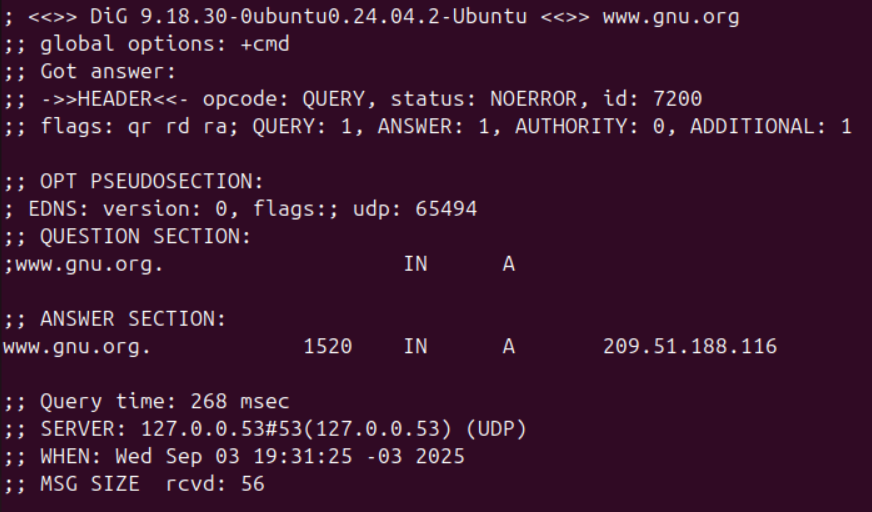
\includegraphics[width=1\linewidth]{Fotos/PrimerDig.png}
    \caption{dig www.gnu.org}
\end{figure}

\begin{figure}
    \centering
    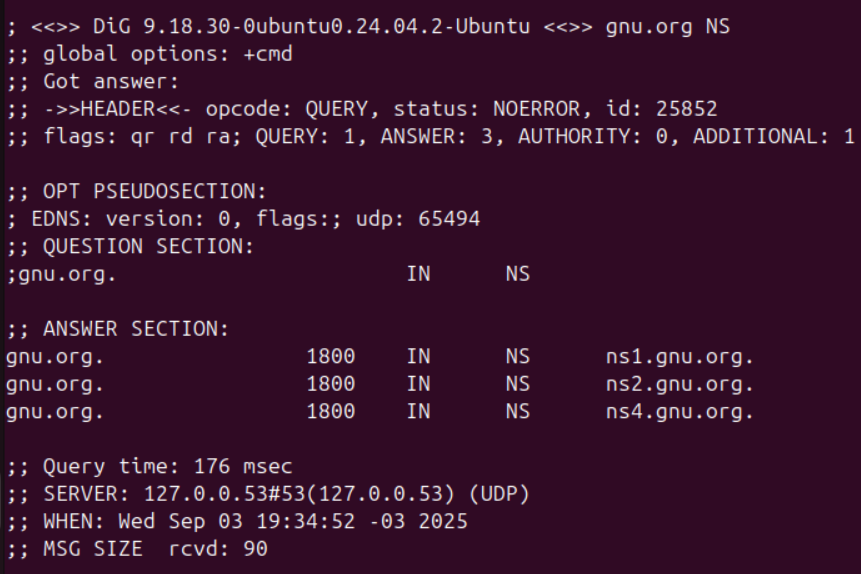
\includegraphics[width=1\linewidth]{Fotos/SegundoDig.png}
    \caption{dig gnu.org NS}
\end{figure}

\begin{figure}
    \centering
    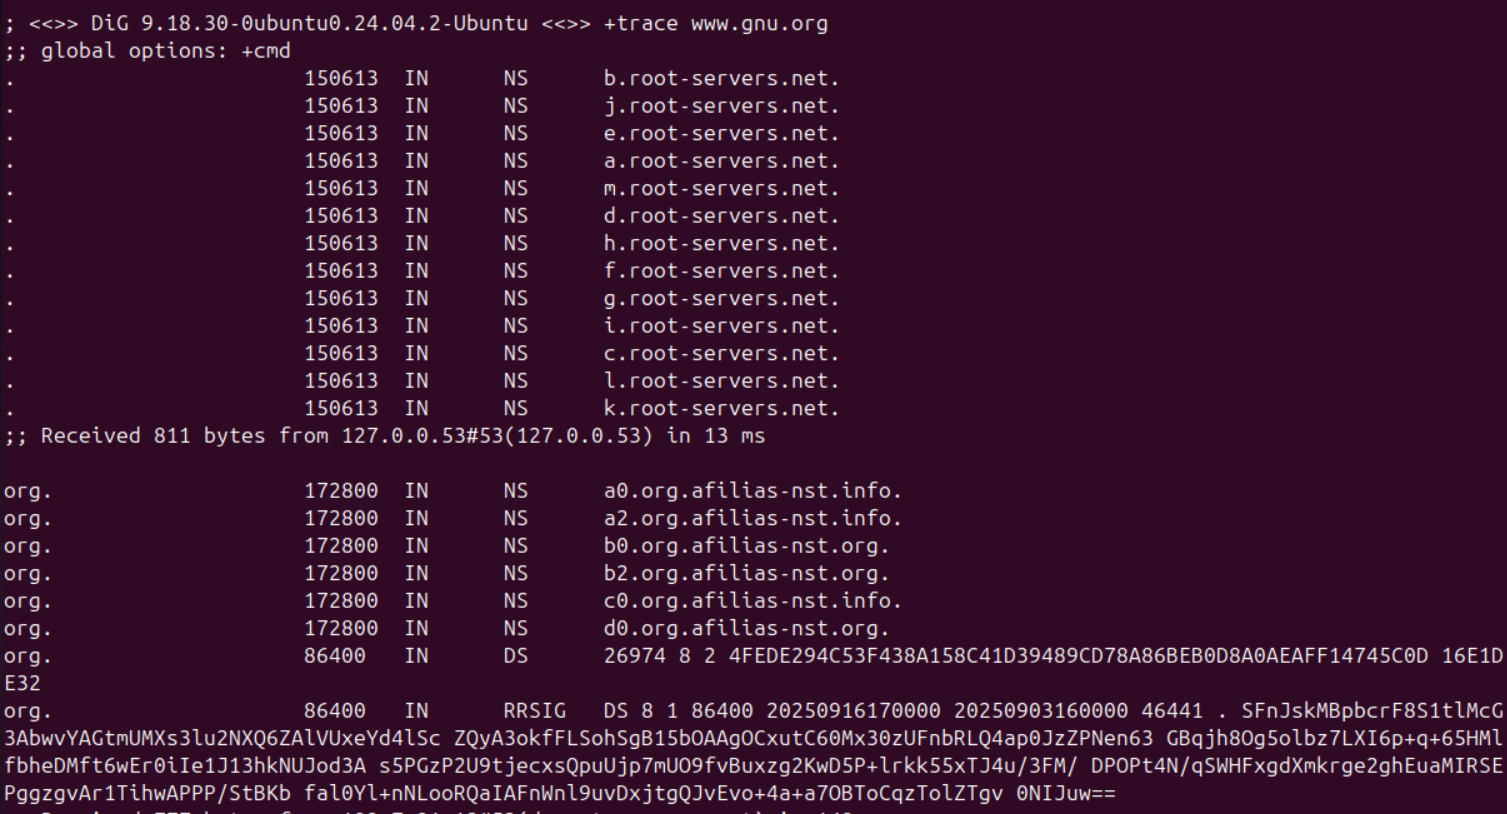
\includegraphics[width=1.25\linewidth]{Fotos/digtrace1.png}
    \caption{dig +trace www.gnu.org primera mitad}
\end{figure}

\begin{figure}
    \centering
    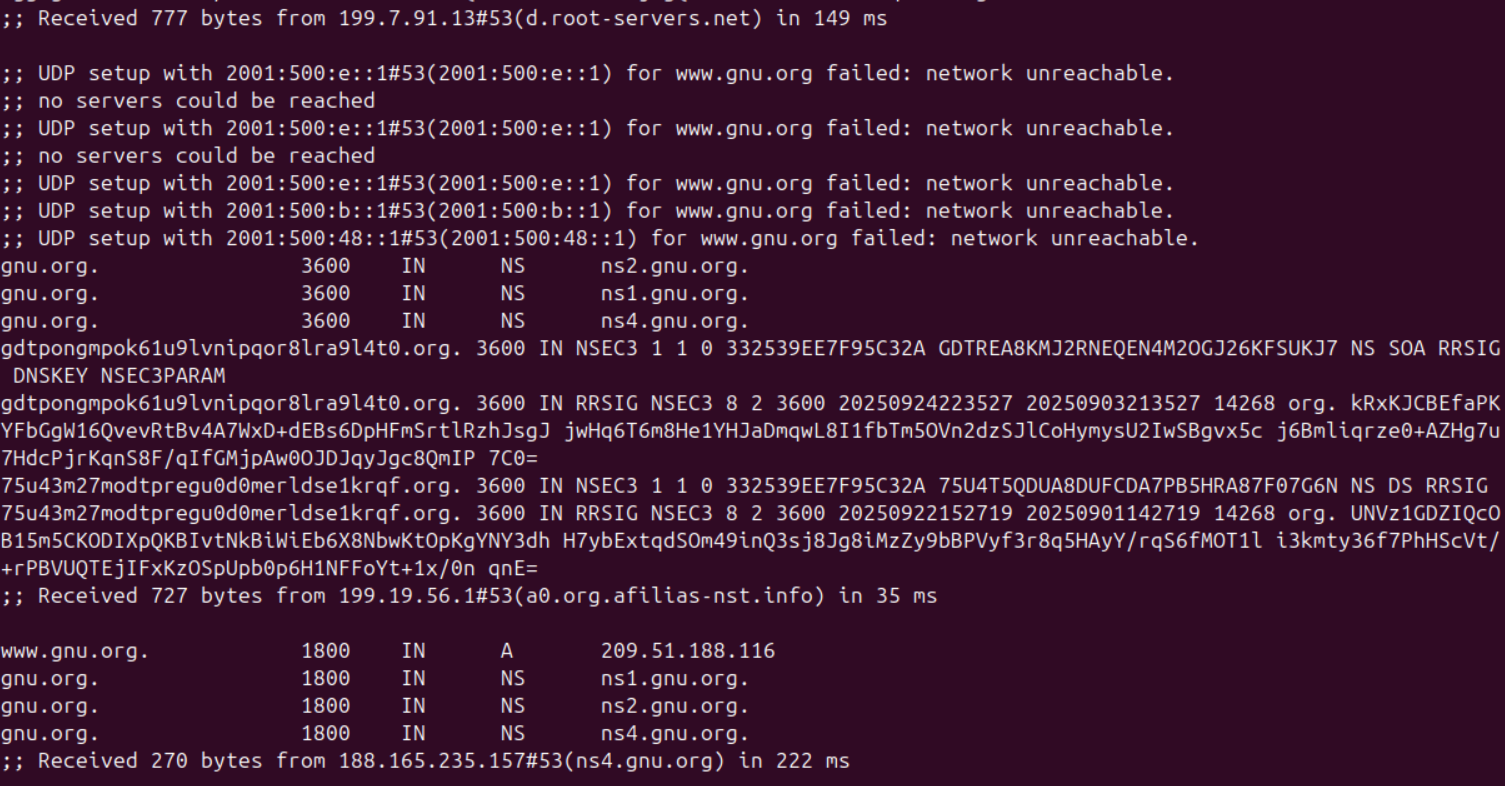
\includegraphics[width=1.25\linewidth]{Fotos/digtrace2.png}
    \caption{dig +trace www.gnu.org segunda mitad}
\end{figure}

En la proxima sección y respondiendo las Cuestiones analizaremos la información brindada por estos comandos.

\newpage

\subsection{Cuestiones}

\subsubsection{Pregunta 1}
El nombre canonico de GNU es www.gnu.org y su direccion ip es 209.51.188.116,esto lo vemos en la primer imagen en la parte de ANSWER SECTION.

\subsubsection{Pregunta 2}
En el resto de la respuesta vemos IN que quiere decir que pertenece a internet la información y 367 que es el tiempo de vida de esta entrada lo que quiere decir que esta información es volátil debido a lo bajo de este valor.

\subsubsection{Pregunta 3}
La dirección ip del servidor DNS que responde la consulta es 127.0.0.53,este servidor es el servidor root que de forma recursiva le pregunta al resto luego por el org  y por el gnu,esta información la sacamos de la primer imagen en la parte SERVER.

\subsubsection{Pregunta 4}
Tener un alias de este servidor DNS es importante para poder ubicarlo,de forma mas sencilla entre todos los que hay ya que cada uno de estos servidores por el mundo se identifican con una letra inicial distinta y todos estos servidores se engloban dentro de una misma ip asi al iniciar la comunicación se pone esa ip y listo y se hacen la consulta a todos los NS disponible,la lista de todos los NS de este server lo vemos en la primer parte de la tercer foto,vemos que se listan 13 servidores.

\subsubsection{Pregunta 5}
Para gnu.org hay tres NS,los cuales se ven en la segunda imagen

\begin{itemize}
\item ns1.gnu.org
\item ns2.gnu.org
\item ns4.gnu.org
\end{itemize}

Luego poniendo el comando dig,sobre cada NS,vamos averiguando sus ip

\begin{itemize}
\item ns1.gnu.org $\rightarrow$  192.99.37.66
\item ns2.gnu.org $\rightarrow$  192.99.35.98
\item ns4.gnu.org $\rightarrow$  188.165.235.157
\end{itemize}



Si vamos a la pagina whois.com vemos que la lista de NS es exactamente la que marcamos recién,confirmando la información,este acceso lo vemos en la imagen 5.

\begin{figure}[h]
    \centering
    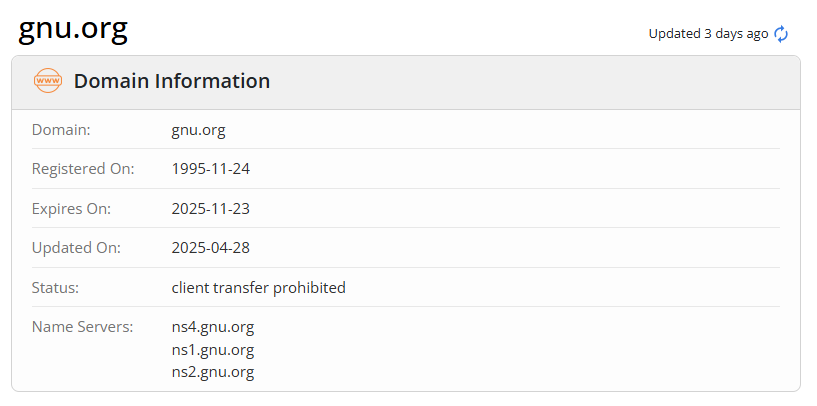
\includegraphics[width=1\linewidth]{Fotos/whoIs.png}
     \caption{Busqueda en whois.com}
\end{figure}

Constatar esta información está bueno para confirmar que existen estos tres NS y que se pueden utilizar de manera confiable.

\subsubsection{Pregunta 6}
Ejecutando el comando,dig +trace www.gnu.org, obtuvimos los NS de los root-servers,de los servers para org, de los para gnu.org y la ip es www.gnu.org además vemos que se utiliza el protocolo de transporte UDP,todo esto esta reflejado en la imagenes 3 y 4 vistas más arriba

\newpage

\section{WireShark}

\subsection{Primer Trama}

Al abrir la primer trame y filtrar los DNS nos quedamos con seis eventos que los vemos en la imagen 6

\begin{figure}[h]
    \centering
    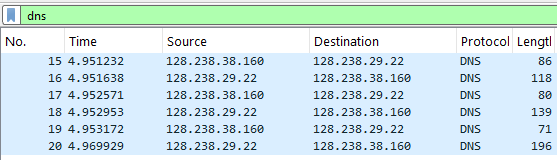
\includegraphics[width=1\linewidth]{Fotos/PrimerTramaEventos.png}
    \caption{Eventos Primer Trama}
\end{figure}

Como dice el TP vamos a centrarnos en los últimos dos eventos de los cuales sacamos la siguiente información,que se analizara en las siguientes preguntas.

\begin{figure}
    \centering
    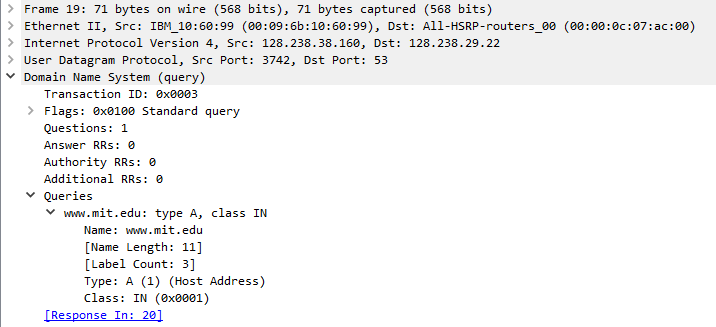
\includegraphics[width=1\linewidth]{Fotos/PrimerTramaPrimerEvento.png}
    \caption{Primer Trama - Penúltimo Evento}
\end{figure}

\begin{figure}[h]
    \centering
    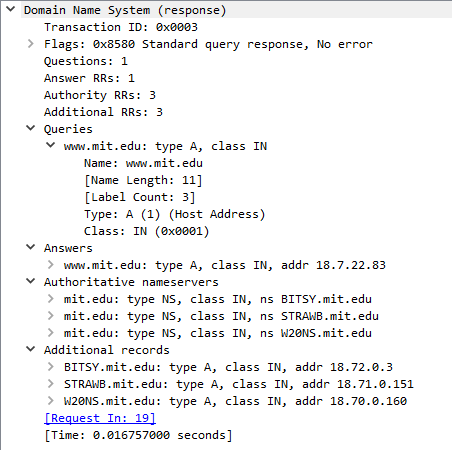
\includegraphics[width=0.75\linewidth]{Fotos/PrimerTramaSegundoEvento.png}
    \caption{Primer Trama - Último Evento}
\end{figure}

\newpage

\subsubsection{Pregunta 1}
DNS utiliza el protocolo de capa de transporte UDP,esto lo vemos en la Imagen 7 donde dice User Datagram Protocol es el protocolo de transporte en el que esta encapsulado.

\subsubsection{Pregunta 2}
El puerto origen de la consulta DNS es 3742 y el destino es 53 en la respuesta será viceversa origen 53 destino 3742,esto se ve en la misma parte que lo de la pregunta 1.

\subsubsection{Pregunta 3}
El paquete DNS es enviado a la dirección 128.238.29.22,como se ve en el destination del penúltimo paquete,esta es la del servidor por defecto según lo dicho en las consignas.

\subsubsection{Pregunta 4}
Hay contenido una pregunta en el mensaje de consulta DNS,la pregunta es de tipo A (host Address),en este caso el campo no contiene ninguna respuesta pero vemos que están dadas las condiciones ya que hay una línea de Answers RRs que en este caso está en 0 osea que no contiene respuestas,todo esto se ve en la Imagen 7.

\subsubsection{Pregunta 5}
En el mensaje de respuesta vemos un Answer que contiene la direccion ip de www.mit.edu que en este caso es 18.7.22.83.
Además vemos los nombres de los NS que tiene el mit.edu,esto en el campo Authoritative nameservers  los cuales son tres:

\begin{itemize}
\item BITSY.mit.edu
\item STRAWB.mit.edu
\item W20NS.mit.edu
\end{itemize}

Y por último en Additional records vemos las direcciones ip de estos tres NS.Estas Son:

\begin{itemize}
\item BITSY.mit.edu $\rightarrow$  18.72.0.3
\item STRAWB.mit.edu $\rightarrow$ 18.71.0.151
\item W20NS.mit.edu $\rightarrow$ 18.70.0.160
\end{itemize}

Toda esta información se ve de forma clara en la Imagen 8.

\newpage

\subsection{Segunda Trama}

En esta segunda trama filtrando en DNS vemos seis eventos,misma cantidad que en trama previa.El trabajo tambien nos pide analizar las últimas dos tramas de las cuales sacamos la información vista en Imagenes 10 y 11 que analizaremos en las preguntas.

\begin{figure}[h]
    \centering
    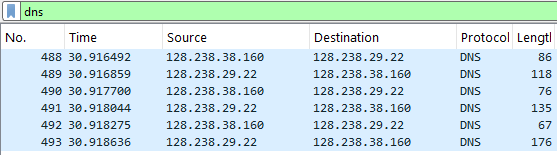
\includegraphics[width=1\linewidth]{Fotos/SegundaTramaEventos.png}
    \caption{Eventos Segunda Trama}
\end{figure}

\begin{figure}
    \centering
    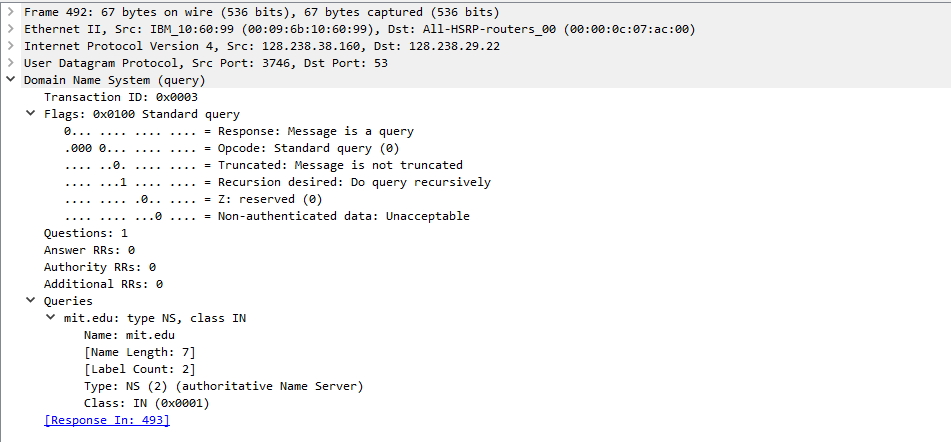
\includegraphics[width=1\linewidth]{Fotos/SegundaTramaPrimerEvento.png}
    \caption{Segunda Trama - Penúltimo Evento}
\end{figure}

\begin{figure}
    \centering
    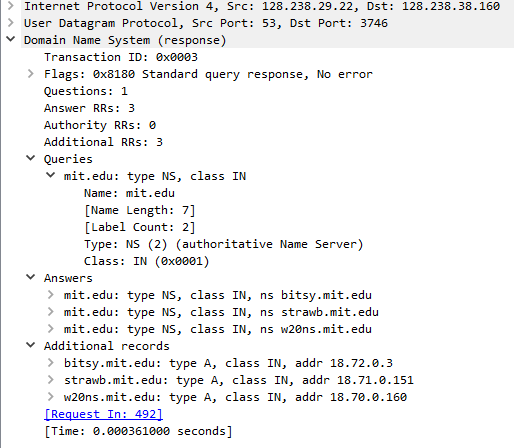
\includegraphics[width=0.75\linewidth]{Fotos/SegundaTramaSegundoEvento.png}
    \caption{Segunda Trama - Último Evento}
\end{figure}

\newpage

\subsubsection{Pregunta 6}
La consulta DNS es enviada a la dirección 128.238.29.22 que es la misma que el servidor local por default,esto se ve en la Imagen 9

\subsubsection{Pregunta 7}
Ahora hay otra vez una pregunta en esta consulta pero esta vez es de tipo 2 (NS)  por lo cual está preguntando por el NS y no por la dirección ip como en el caso anterior,también vemos que el mensaje otra vez puede contener respuestas pero en este caso no las contiene,esto lo vemos en la Imagen 10.

\subsubsection{Pregunta 8}
Vemos que hay respuestas en este caso tres que son los tres NS que mencionamos anteriormente en la consigna 5,también en adicional hay tres respuestas que son las tres direcciones ip mencionadas también la consigna 5,lo que no hay es campo authority ya que en este caso eso se contesta en la misma respuesta ya que es la pregunta a responder,esto lo vemos en la Imagen 11

\newpage
\subsection{Comando nslookup}

Ejecutando el comando,nslookup -sil -type=NS mit.edu, nos encontramos con sorpresas:

\begin{figure}[h]
    \centering
    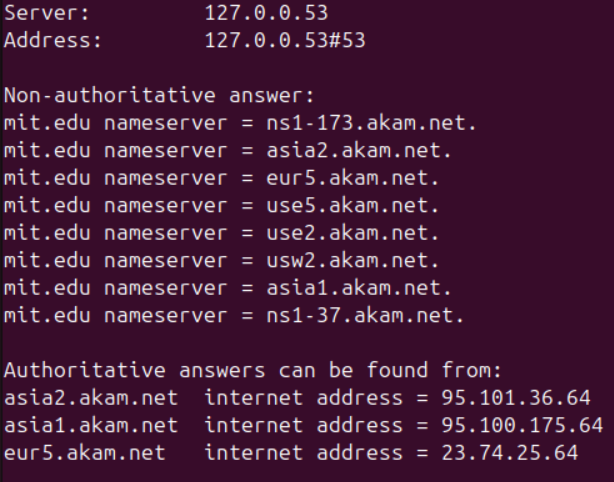
\includegraphics[width=0.5\linewidth]{Fotos/nslookup.png}
    \caption{comando nslookup -sil -type=NS mit.edu}
\end{figure}

Lo más notorio es que los NS listados no coinciden con los vistos en las preguntas,esto se puede atribuir al paso del tiempo capaz desde el armado de la trama a la actualidad hubo un cambio en estos,creandose nuevos y renombrando los anteriores,tambien vemos que el servidor DNS no coincide con el dado en la trama aunque eso puede deberse mas a que quiza en la terminal nos indica otro servidor.

Lo importante de esto es que vemos como el DNS cambia a través del tiempo sufriendo modificaciones en sus NS,Ips,entre otras cosas,pero el principal DNS,que es mit.edu en este caso, no ha cambiado por lo que estos cambios no afectan en si a los usuarios si no es más una cuestión interna.
\end{document}
